% Proposta de gráfico com uma série de preços de exemplo, para a seção 1.4 do TG
% (13/11/2026, pedido do autor). NÃO é parte do TG. Dados em
% dados/resultados/serie_exemplo_2026-11-13/ (ferramentas/scripts/serie_exemplo.sh).
\documentclass[11pt,a4paper]{article}
\usepackage[T1]{fontenc}
\usepackage[brazilian]{babel}
\usepackage{mathptmx}
\usepackage[a4paper,margin=2.4cm]{geometry}
\usepackage{graphicx}
\usepackage[font=small,labelfont=bf]{caption}
\usepackage[most]{tcolorbox}
\usepackage[hidelinks]{hyperref}
\setlength{\parskip}{0.45em}
\setlength{\parindent}{0pt}
\definecolor{cmod}{RGB}{0,90,181}
\newtcolorbox{ideia}[1][]{colback=cmod!5, colframe=cmod!70, fonttitle=\bfseries, title={#1}, arc=2pt, boxrule=0.6pt}

\title{Uma série de preços de exemplo\\[2pt]\large proposta de gráfico para a seção 1.4}
\author{Material de análise, fora do TG}
\date{13 de novembro de 2026}

\begin{document}
\maketitle

A seção 1.4, Modelos estatísticos de séries temporais, começa dizendo que os
fechamentos de uma ação, um por pregão, formam uma série temporal, e que as séries
financeiras costumam ser estudadas pelo retorno, a variação de um dia para o outro.
Hoje isso está só em palavras. As duas propostas abaixo mostram a série de verdade,
com a PETR4 da própria base do trabalho (o COTAHIST da B3), sem nenhum número
digitado: os dados saem do script \texttt{ferramentas/scripts/serie\_exemplo.sh}.

\section{Proposta A: os últimos 20 pregões}

\begin{center}
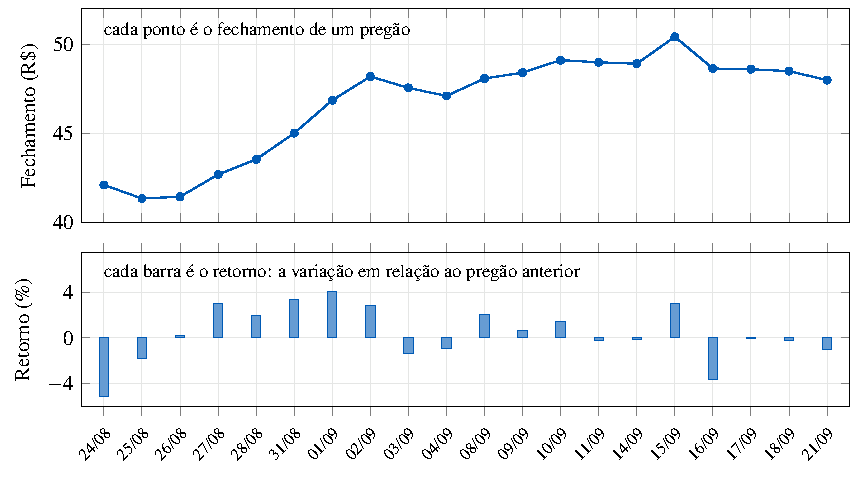
\includegraphics[width=\linewidth]{fig-serie-curta.pdf}
\end{center}

Os 20 últimos pregões da série, de 24/08/2026 a 21/09/2026. Em cima, cada ponto é um
fechamento. Embaixo, cada barra é o retorno daquele pregão em relação ao anterior.
Com poucos pontos, dá para ver que a série é uma sequência de valores, um por
pregão, e que o retorno é outra série, feita das variações da primeira. É
exatamente o que os dois primeiros parágrafos da 1.4 dizem.

\section{Proposta B: 2019 a 2021}

\begin{center}
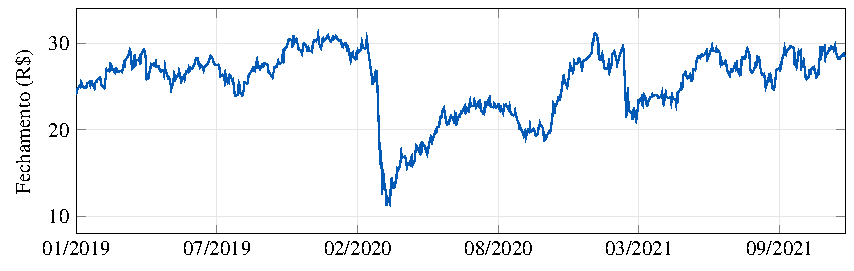
\includegraphics[width=\linewidth]{fig-serie-longa.pdf}
\end{center}

O fechamento de 2019 a 2021, o mesmo período do Gráfico~1 do TG, que mostra os
retornos dessa mesma série. Ela ilustra o terceiro parágrafo da 1.4: o preço anda
sem rumo definido e não volta a uma média, como na queda de 2020 e na recuperação
que veio depois. Lida junto com o Gráfico~1, mostra o preço e o retorno do mesmo
período.

\begin{ideia}[Recomendação: a proposta A]
A A ensina os dois conceitos que a 1.4 apresenta primeiro, série e retorno, e não
repete o período do Gráfico~1. A B serve melhor para o ``passeio aleatório'', mas
o Gráfico~1 já mostra esse período, e a figura sozinha fala mais da pandemia do que
da série. Se quiser as duas ideias, a B pode ficar para os slides.
\end{ideia}

\section{Se entrar no TG}

Pela norma é um \textbf{Gráfico} (representação geométrica de dados), com título em
cima, fonte embaixo e citação no texto. Lugar sugerido: logo depois do parágrafo do
retorno, na 1.4. Por exemplo:

\begin{itemize}
\item Título: ``Gráfico~1 -- Fechamento e retorno da PETR4 nos últimos 20 pregões da
  série''. Ele passaria a ser o Gráfico~1, e os demais andam um número.
\item Fonte: ``Elaboração própria com dados de B3 (2026).'', como no gráfico da
  heterocedasticidade.
\item Frase que o chama: ``O Gráfico~1 mostra um trecho da série de fechamentos da
  PETR4 e o retorno de cada pregão.''
\end{itemize}

O gráfico tem cerca de meia página. Ao inserir, rodar de novo o
\texttt{checar\_ilustracoes.sh} e conferir se não sobra página em branco.

\end{document}
